\documentclass{article}
\usepackage{graphicx}
\usepackage{tikz}
\begin{document}

\begin{center}

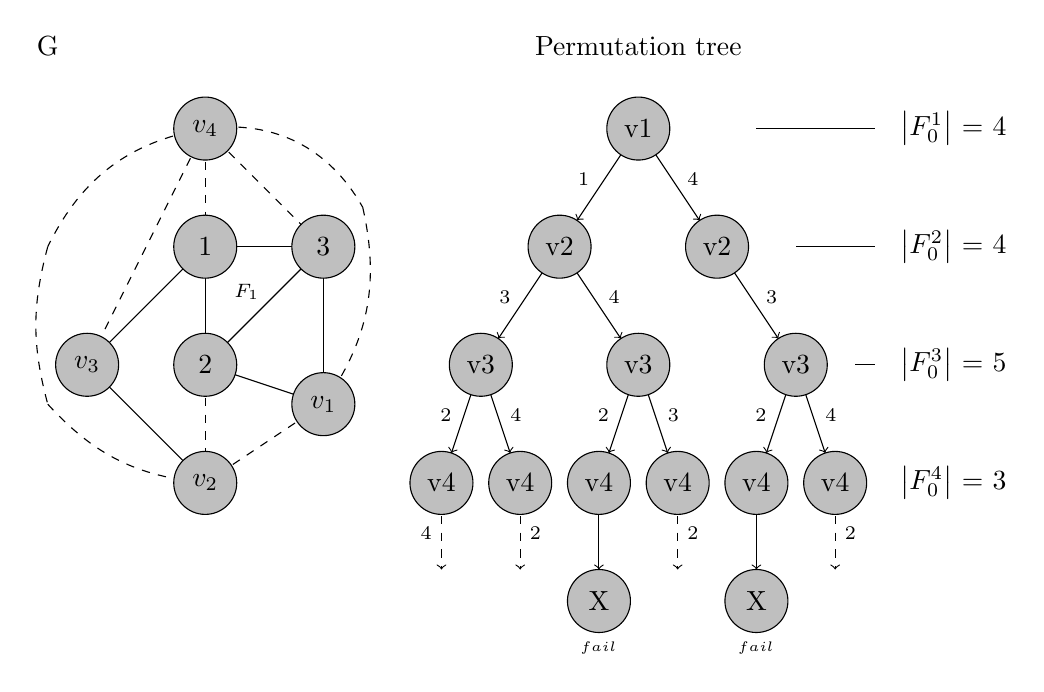
\begin{tikzpicture}
\draw[above, yshift=0.8cm] (1,13.5) node{G}; % Graph title
  \draw[dashed] (3,13.5) to[bend left=34] (5,12.5); % v4 -- (5,12.5)
  \draw[dashed] (3,13.5) to[bend right=27] (1,12); % v4 -- (1,12)
  \draw[dashed] (3,13.5) -- (3,12); % v4 -- 1
  \draw[dashed] (3,13.5) -- (4.5,12); % v4 -- 3
  \draw[dashed] (3,13.5) -- (1.5,10.5); % v4 -- v3
  \draw[dashed] (5,12.5) to[bend left=24] (4.5,10); % (5,12.5) -- v1
  \draw[dashed] (1,12) to[bend right=15] (1,10); % (1,12) -- (1,10)
  \draw (3,12) -- (4.5,12); % 1 -- 3
  \draw (3,12) -- (1.5,10.5); % 1 -- v3
  \draw (3,12) -- (3,10.5)
  node[midway, xshift=15pt, yshift=5pt]{\scriptsize $F_1$}
  ; % 1 -- 2
  \draw (4.5,12) -- (3,10.5); % 3 -- 2
  \draw (1.5,10.5) -- (3,9); % v3 -- v2
  \draw (3,10.5) -- (4.5,10); % 2 -- v1
  \draw[dashed] (3,10.5) -- (3,9); % 2 -- v2
  \draw[dashed] (1,10) to[bend right=21] (3,9); % (1,10) -- v2
  \draw (4.5,10) -- (4.5,12); % v1 -- 3
  \draw[dashed] (3,9) -- (4.5,10); % v2 -- v1
  \filldraw[fill=lightgray] (3,13.5) circle (0.4) node{$v_4$};
  \filldraw[fill=lightgray] (3,12) circle (0.4) node{1};
  \filldraw[fill=lightgray] (4.5,12) circle (0.4) node{3};
  \filldraw[fill=lightgray] (1.5,10.5) circle (0.4) node{$v_3$};
  \filldraw[fill=lightgray] (3,10.5) circle (0.4) node{2};
  \filldraw[fill=lightgray] (4.5,10) circle (0.4) node{$v_1$};
  \filldraw[fill=lightgray] (3,9) circle (0.4) node{$v_2$};
    
    % GRAFO AP
  \draw[above, yshift=0.8cm] (8.5,13.5) node{Permutation tree}; % Graph title
  \draw[->, shorten >=0.4cm] (8.5,13.5) -- (7.5,12)
   node[midway, left, yshift=3pt]{\scriptsize 1}
  ; % v1 -> v2
  \draw[->, shorten >=0.4cm] (8.5,13.5) -- (9.5,12)
  node[midway, right, yshift=3pt]{\scriptsize 4}
  ; % v1 -> v2
  \draw[->, shorten >=0.4cm] (7.5,12) -- (6.5,10.5)
  node[midway, left, yshift=3pt]{\scriptsize 3}
  ; % v2 -> v3
  \draw[->, shorten >=0.4cm] (7.5,12) -- (8.5,10.5)
  node[midway, right, yshift=3pt]{\scriptsize 4}
  ; % v2 -> v3
  \draw[->, shorten >=0.4cm] (9.5,12) -- (10.5,10.5)
  node[midway, right, yshift=3pt]{\scriptsize 3}
  ; % v2 -> v3
  \draw[->, shorten >=0.4cm] (6.5,10.5) -- (6,9)
  node[midway, left, yshift=3pt]{\scriptsize 2}
  ; % v3 -> v4
  \draw[->, shorten >=0.4cm] (6.5,10.5) -- (7,9)
  node[midway, right, yshift=3pt]{\scriptsize 4}
  ; % v3 -> v4
  \draw[->, shorten >=0.4cm] (8.5,10.5) -- (8,9)
  node[midway, left, yshift=3pt]{\scriptsize 2}
  ; % v3 -> v4
  \draw[->, shorten >=0.4cm] (8.5,10.5) -- (9,9)
  node[midway, right, yshift=3pt]{\scriptsize 3}
  ; % v3 -> v4
  \draw[->, shorten >=0.4cm] (10.5,10.5) -- (10,9)
  node[midway, left, yshift=3pt]{\scriptsize 2}
  ; % v3 -> v4
  \draw[->, shorten >=0.4cm] (10.5,10.5) -- (11,9)
  node[midway, right, yshift=3pt]{\scriptsize 4}
  ; % v3 -> v4
  \draw[dashed, ->, shorten >=0.4cm] (6,9) -- (6,7.5)
  node[midway, left, yshift=3pt]{\scriptsize 4}
  ; % v4 -> (6,7.5)
  \draw[dashed, ->, shorten >=0.4cm] (7,9) -- (7,7.5)
  node[midway, right, yshift=3pt]{\scriptsize 2}
  ; % v4 -> (7,7.5)
  \draw[->, shorten >=0.4cm] (8,9) -- (8,7.5); % v4 -> X
  \draw[dashed, ->, shorten >=0.4cm] (9,9) -- (9,7.5)
  node[midway, right, yshift=3pt]{\scriptsize 2}
  ; % v4 -> (9,7.5)
  \draw[->, shorten >=0.4cm] (10,9) -- (10,7.5); % v4 -> X
  \draw[dashed, ->, shorten >=0.4cm] (11,9) -- (11,7.5)
  node[midway, right, yshift=3pt]{\scriptsize 2}
  ; % v4 -> (11,7.5)
  \filldraw[fill=lightgray] (8.5,13.5) circle (0.4) node{v1};
  \filldraw[fill=lightgray] (7.5,12) circle (0.4) node{v2};
  \filldraw[fill=lightgray] (9.5,12) circle (0.4) node{v2};
  \filldraw[fill=lightgray] (6.5,10.5) circle (0.4) node{v3};
  \filldraw[fill=lightgray] (8.5,10.5) circle (0.4) node{v3};
  \filldraw[fill=lightgray] (10.5,10.5) circle (0.4) node{v3};
  \filldraw[fill=lightgray] (6,9) circle (0.4) node{v4};
  \filldraw[fill=lightgray] (7,9) circle (0.4) node{v4};
  \filldraw[fill=lightgray] (8,9) circle (0.4) node{v4};
  \filldraw[fill=lightgray] (9,9) circle (0.4) node{v4};
  \filldraw[fill=lightgray] (10,9) circle (0.4) node{v4};
  \filldraw[fill=lightgray] (11,9) circle (0.4) node{v4};
  \filldraw[fill=lightgray] (8,7.5) circle (0.4) node{X}
  node[below, yshift=-0.4cm]{\scriptsize $_{fail}$}
  ;
  \filldraw[fill=lightgray] (10,7.5) circle (0.4) node{X}
  node[below, yshift=-0.4cm]{\scriptsize $_{fail}$}
  ;
  \draw (12.5,13.5) node{$\left| F_{0}^{1} \right|$ = 4};
  \draw (11.5,13.5) -- (10,13.5);
  \draw (12.5,12) node{$\left| F_{0}^{2} \right|$ = 4};
  \draw (11.5,12) -- (10.5,12);
  \draw (12.5,10.5) node{$\left| F_{0}^{3} \right|$ = 5};
  \draw (11.5,10.5) -- (11.25,10.5);
  \draw (12.5,9) node{$\left| F_{0}^{4} \right|$ = 3};
\end{tikzpicture}


\end{center}
\end{document}
